A model that predicts functional magnetic resonance imaging (fMRI) from electroencephalography (EEG) would give access to haemodynamic information at the cost and in the settings of an EEG recording. Deep synthesizers \citep{liu2019convolutional,calhas2022eeg,li2024neurobolt} have been proposed for this, and for any clinical use their predictions need an uncertainty estimate \citep{begoli2019need}. Uncertainty quantification (UQ) can be done through heteroscedastic likelihoods \citep{kendall2017uncertainties}, approximate Bayesian weights \citep{blundell2015weight,gal2016dropout,maddox2019simple,daxberger2021laplace}, ensembles \citep{lakshminarayanan2017simple} and conformal intervals \citep{lei2018distribution,romano2019conformalized}. 

EEG-to-fMRI synthesis is an unusual setting for these tools. Most of the variance of an fMRI volume is anatomy shared across subjects, learnable without the EEG, and the part that varies in time also follows the heart and head motion, which leak into the EEG \citep{friston1996movement,power2014methods}. A predictive distribution can therefore be calibrated, its spread can track its error, and its mean can pass a surrogate test, while it carries no neural information from the EEG. The standard checks never ask what they give without the input. \citet{liu2019convolutional} first mapped EEG to fMRI volumes with a convolutional network, and \citet{calhas2022eeg} proposed the encoder we use. In medical imaging, uncertainty has been studied for segmentation \citep{mehrtash2020confidence}, reconstruction \citep{narnhofer2021bayesian} and diffusion MRI \citep{tanno2021uncertainty}, where the target is mostly determined by the input, so whether the uncertainty depends on the input need not be asked. Our protocol carries the negative controls of neuroimaging machine learning \citep{varoquaux2018cross,kapoor2023leakage,schreiber1996improved} over to predictive uncertainty.

\begin{figure}[!htbp]
    \centering
    
    \begin{tikzpicture}
        [scale=1.2, inner sep=3mm,
        in_node/.style={circle, draw=red!90, fill=red!20,thick,inner sep=0pt, minimum size=3mm},
        out_node/.style={circle, draw=blue!90, fill=blue!20,thick,inner sep=0pt,minimum size=3mm}]
            
        
        %draw model 1st model
        %in nodes
        \node (1stinnode) at (0,0) [in_node] {};
        \node (2ndinnode) at ($(1stinnode)+(0.5,0)$) [in_node] {};
        \node (3rdinnode) at ($(2ndinnode)+(0.5,0)$) [in_node] {};
        %out nodes
        \node (3rdoutnode) at ($(2ndinnode)+(0,1)$) [out_node] {};
        \node (1stoutnode) at ($(3rdoutnode)+(-1,0)$) [out_node] {};
        \node (2ndoutnode) at ($(1stoutnode)+(0.5,0)$) [out_node] {};
        \node (3rdoutnode) at ($(2ndoutnode)+(0.5,0)$) [out_node] {};
        \node (4thoutnode) at ($(3rdoutnode)+(0.5,0)$) [out_node] {};
        \node (5thoutnode) at ($(4thoutnode)+(0.5,0)$) [out_node] {};
        %fully connect nodes
        \draw[->] (1stinnode) -- (1stoutnode);
        \draw[->] (1stinnode) -- (2ndoutnode);
        \draw[->] (1stinnode) -- (3rdoutnode);
        \draw[->] (1stinnode) -- (4thoutnode);
        \draw[->] (1stinnode) -- (5thoutnode);
        \draw[->] (2ndinnode) -- (1stoutnode);
        \draw[->] (2ndinnode) -- (2ndoutnode);
        \draw[->] (2ndinnode) -- (3rdoutnode);
        \draw[->] (2ndinnode) -- (4thoutnode);
        \draw[->] (2ndinnode) -- (5thoutnode);
        \draw[->] (3rdinnode) -- (1stoutnode);
        \draw[->] (3rdinnode) -- (2ndoutnode);
        \draw[->] (3rdinnode) -- (3rdoutnode);
        \draw[->] (3rdinnode) -- (4thoutnode);
        \draw[->] (3rdinnode) -- (5thoutnode);
        %prediction
        %left lower right upper
        \node (1stprediction) at ($(3rdoutnode)+(0,2.8)$) {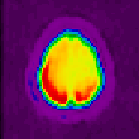
\includegraphics[width=0.17\textwidth]{figures/intro/full_pred.pdf}};
        \draw[->, ultra thick, draw=blue] ($(3rdoutnode)+(0,0.5)$) -- ($(1stprediction)+(0,-1.8)$);
        %x
        \node (input) at ($(2ndinnode)+(0,-2)$) {};
        \node (raw) at ($(input)+(-1.,0)$) {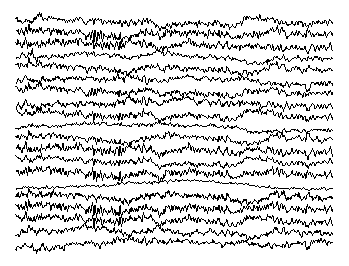
\includegraphics[width=0.08\textwidth]{figures/intro/eeg.pdf}};
        \node (stft) at ($(input)+(1.,0)$) {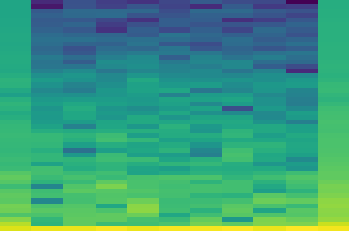
\includegraphics[width=0.09\textwidth]{figures/intro/stft.pdf}};
        \draw[->] ($(raw)+(0.7,0)$) -- ($(stft)+(-0.8,0)$);
        \draw[->, ultra thick, draw=blue] ($(input)+(0,1.1)$) -- ($(2ndinnode)+(0,-0.4)$);

        \node (eeg_legend) at ($(input)+(-3.5,0)$) {};
        \node[align=center] at ($(input)+(-3.7,0)$) {EEG recording\\Time frequency\\STFT domain};
        \node (model_legend) at ($(2ndinnode)+(-3.5,0.5)$) {Model};
        \node (fmri_legend) at ($(1stprediction)+(-3.5,0)$) {fMRI prediction};
        %table like lines
        \draw[dotted, opacity=0.8] ($(eeg_legend)+(-2,1.3)$) -- ($(eeg_legend)+(11.8,1.3)$);
        \draw[dotted, opacity=0.8] ($(model_legend)+(-2,1.15)$) -- ($(model_legend)+(11.8,1.15)$);

        
        
        %draw model 2nd 
        %in nodes
        \node (1stinnode) at ($(1stinnode)+(6.5,0)$) [in_node] {};
        \node (2ndinnode) at ($(1stinnode)+(0.5,0)$) [in_node] {};
        \node (3rdinnode) at ($(2ndinnode)+(0.5,0)$) [in_node] {};
        %out nodes
        \node (2ndoutnode) at ($(2ndinnode)+(0,1)$) [out_node] {};
        \node (3rdoutnode) at ($(2ndoutnode)+(0.5,0)$) [out_node] {};
        \node (1stoutnode) at ($(3rdoutnode)+(-1,0)$) [out_node] {};
        %fully connect nodes
        \draw[->] (1stinnode) -- (1stoutnode);
        \draw[->] (1stinnode) -- (2ndoutnode);
        \draw[->] (1stinnode) -- (3rdoutnode);
        \draw[->] (2ndinnode) -- (1stoutnode);
        \draw[->] (2ndinnode) -- (2ndoutnode);
        \draw[->] (2ndinnode) -- (3rdoutnode);
        \draw[->] (3rdinnode) -- (1stoutnode);
        \draw[->] (3rdinnode) -- (2ndoutnode);
        \draw[->] (3rdinnode) -- (3rdoutnode);
        %prediction
        \node (2ndprediction) at ($(2ndoutnode)+(0,2.8)$) {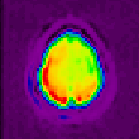
\includegraphics[width=0.17\textwidth]{figures/intro/relaxed_pred.pdf}};
        \draw[->, ultra thick, draw=blue] ($(2ndoutnode)+(0,0.5)$) -- ($(2ndprediction)+(0,-1.8)$);
        %eeg x
        \node (input) at ($(2ndinnode)+(0,-2)$) {};
        \node (raw) at ($(input)+(-1.,0)$) {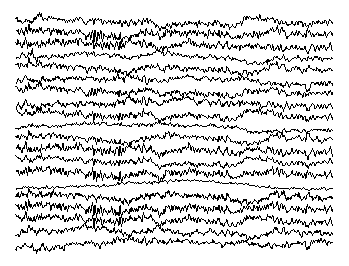
\includegraphics[width=0.08\textwidth]{figures/intro/eeg.pdf}};
        \node (stft) at ($(input)+(1.,0)$) {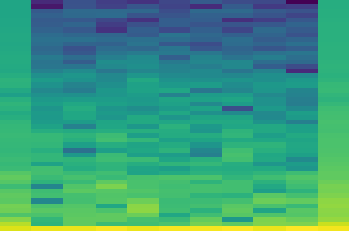
\includegraphics[width=0.09\textwidth]{figures/intro/stft.pdf}};
        \draw[->] ($(raw)+(0.7,0)$) -- ($(stft)+(-0.8,0)$);
        \draw[->, ultra thick, draw=blue] ($(input)+(0,1.1)$) -- ($(2ndinnode)+(0,-0.4)$);
        %problem relaxation
        \draw[->, ultra thick] ($(5thoutnode)+(0.5,0.5)$) -- ($(1stoutnode)+(-0.5,0.5)$);
        \node[align=center] (description) at ($(5thoutnode)+(2.45,-0.5)$) {predict less\\features};

        \node at ($(fmri_legend)+(0,2.1)$) {Resolution};
        \node at ($(1stprediction)+(0,2.1)$) {full};
        \node at ($(2ndprediction)+(0,2.1)$) {lower};
        \draw[opacity=0.4] ($(fmri_legend)+(-2,1.7)$) -- ($(fmri_legend)+(11.8,1.7)$);

        \node at ($(1stprediction)+(2.3,0.8)$) {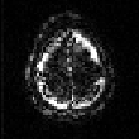
\includegraphics[width=0.065\textwidth]{figures/intro/full_res.pdf}};
        \node at ($(2ndprediction)+(-2.3,0.8)$) {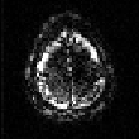
\includegraphics[width=0.065\textwidth]{figures/intro/relaxed_res.pdf}};
        
    \end{tikzpicture}
    \caption{EEG-to-fMRI synthesis and the spectral relaxation. EEG windows are transformed to the time--frequency (STFT) domain and mapped to an fMRI volume. The relaxed decoder predicts only the low spatial frequencies of the volume (fewer outputs, right) instead of the full resolution (left), consistent with the low spatial resolution of the EEG. The predictions are real outputs for a CHUR-XP2 test subject (axial slice 20): the stochastic spectral decoder, whose samples span the full resolution (left), and the zero-filled heteroscedastic network (right); the small grey maps beside them are their absolute residues; we also quantify what such a relaxed decoder can and cannot express.}
    \label{fig:idea_description}
\end{figure}


This study asks whether the uncertainty of EEG-to-fMRI synthesizers is about the EEG. To this end, our contributions are:
\begin{itemize}
	\item \textbf{An EEG-conditional evaluation protocol.} A model must beat EEG-free predictive distributions, and must change when its EEG is shifted in time or swapped across subjects (see Sec. \ref{sec:problem}).
	\item \textbf{A benchmark of eleven UQ methods} on a shared backbone, including our stochastic spectral decoder built on a DCT relaxation of the decoder. None beats an EEG-free template, and their uncertainty is a static anatomical map (see Sec. \ref{sec:methods}).
	\item \textbf{A positive control} showing that the heteroscedastic training most methods share makes the network ignore its input (see Sec. \ref{sec:results}).
	\item \textbf{A region-level analysis} in which an EEG model passes the surrogate test of \citet{mehta2025eegbold}, but heart rate from the in-scanner ECG predicts as much, and across subjects the EEG adds nothing to heart rate and motion (see Sec. \ref{sec:results}).
\end{itemize}
The results concern two motor-imagery datasets and the models we tested; they do not say that EEG carries no haemodynamic information \citep{goldman2002simultaneous,laufs2003eeg}.
